% ============================================================================
% entropybrush — digital-twin paper (arXiv v1 draft)
%   Build: tectonic main.tex   (TEST pdflatex before arXiv; ship main.bbl)
%   Scope (v1): a design + simulation-validated systems paper. The physical
%   demonstrator is NOT built; every claim about physical output is future work.
% ============================================================================
\documentclass[11pt]{article}

\usepackage[margin=1.1in]{geometry}
\usepackage[T1]{fontenc}
\usepackage[utf8]{inputenc}
\usepackage{lmodern}
\usepackage{microtype}
\usepackage{amsmath}
\usepackage{booktabs}
\usepackage{graphicx}
\usepackage{siunitx}
\usepackage{tikz}
\usetikzlibrary{positioning,arrows.meta}
\usepackage[numbers,sort&compress]{natbib}
\usepackage[hidelinks]{hyperref}

% Absorb the occasional overfull line from long \texttt{} tokens (code names)
% without hyphenating code across lines.
\emergencystretch=2em

\newcommand{\figplaceholder}[2]{%
  \fbox{\parbox[c][11em][c]{0.92\linewidth}{\centering\small
    \textbf{[figure placeholder]}\\[0.6em]#1\\[0.8em]\texttt{\footnotesize #2}}}}
\newcommand{\code}[1]{\texttt{\small #1}}

\title{\textbf{Painting as a Deterministic Performance:\\
A Physics-Based Simulation Twin and Machine-Agnostic Interface\\
for Physical Painting Machines}}
\author{Dan Newcome\\[2pt]
  \small entropybrush\\
  \small\texttt{<email TODO>} \quad \small\url{https://github.com/dnuke-art/entropy-brush}}
\date{July 2026 --- draft (arXiv v1)}

\begin{document}
\maketitle

\begin{abstract}
Physically-based painting simulators reproduce the look of oil and watercolour
on screen, and painting robots execute planned strokes with real media, but the
two are rarely coupled: the simulator's paint physics does not usually author the
machine's motion, and the machine does not usually consume a physics-grounded
description of the intended painting. We argue that a paint simulator is most
useful to a physical painting machine when the system is factored at a
\emph{machine-agnostic performance interface} --- a deterministic, replayable
stream of brush \emph{intent} (position, contact pressure, and pigment), not
kinematics --- and when the simulated impasto height field is reused directly as
\emph{fabrication geometry}. We describe entropybrush, an open-source
height-field oil-paint simulator built around this factoring, and its
\code{TwinPerformance} interface and dual-use height field. We are explicit about
evidence class: determinism of the performance stream, conservation of the paint
mass, and watertightness of the exported relief mesh are \emph{simulation-%
validated} (headless tests); the paint model itself is a re-implementation of
established techniques and is \emph{not} claimed as novel. The central systems
claim --- that this interface lets a simulator faithfully drive a physical
painting --- is \emph{not yet demonstrated}: no machine has executed a
performance. This paper presents the design and its simulation-level validation;
the physical loop, and a simulation-versus-physical fidelity study, are stated
future work.
\end{abstract}

\begin{figure}[t]
\centering
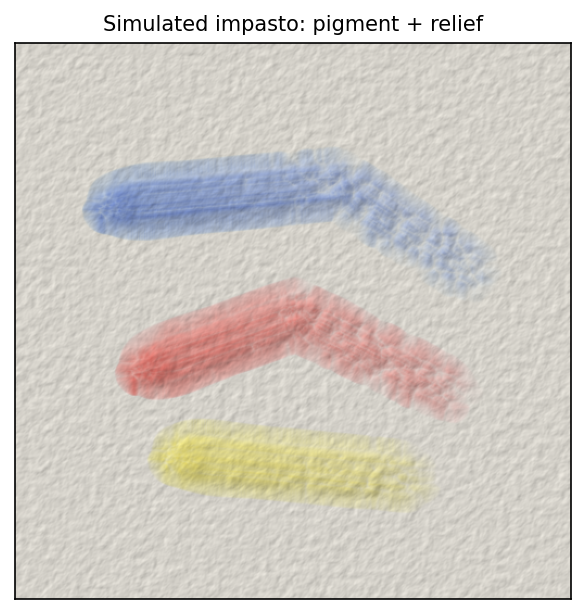
\includegraphics[width=0.58\linewidth]{figures/impasto_relief.png}
\caption{A painting made in entropybrush, shown as its simulated relief: pigment
(Kubelka--Munk) over a physically-simulated impasto height field, with bristle
striations and drybrush tails. The same field is reused as fabrication geometry
(Figure~\ref{fig:dual}). Rendered \emph{offline} from the sim's height and albedo
fields (\code{tools/paper\_figs.dart} $+$ \code{figures/gen\_figures.py}); the
in-app GPU shader render is richer.}
\label{fig:teaser}
\end{figure}

\section{Introduction}

Two mature bodies of work bracket this paper. On one side, physically-based
digital painting has, for more than two decades, modelled paint as a fluid on a
height field with pigment optics and brush dynamics, from watercolour
\citep{curtis1997watercolor} through interactive oil paint
\citep{baxter2004impasto,chen2015wetbrush,stuyck2016oilmobile}. On the other,
painting machines execute strokes with real media under visual or planned
control. What is comparatively rare is a \emph{coupling} in which the paint
physics is the authoring front-end for the machine, and the machine consumes a
physics-grounded, reproducible description of the intended painting rather than a
bare toolpath.

We take the position that the useful coupling is an \emph{interface}, not a
monolith. A painting can be recorded as a deterministic \emph{performance}: a
timestamped stream of brush \emph{intent} --- where the brush went, how hard, and
in what colour --- deliberately free of kinematics, firmware, or a paint-well
map. The simulator is then a \emph{twin}: it authors the performance, previsualises
its result, and (because replay is deterministic at the op level) specifies it
reproducibly, while a separate machine driver owns everything hardware. A second
consequence falls out of a height-field paint model: the impasto relief that is
shaded on screen \emph{is} a surface, so the same field exports directly as a
watertight, millimetre-scaled mesh --- the preview and the fabrication geometry
are one representation.

\paragraph{Contributions.} We claim, and support at the evidence class stated for
each:
\begin{enumerate}
\item \textbf{A machine-agnostic performance interface} for painting
  (Section~\ref{sec:interface}): an ordered, versioned stream of brush intent
  (position, pressure$\rightarrow$Z, pigment), with an explicit simulator/hardware
  boundary that keeps kinematics and firmware out of the authoring tool.
  \emph{(Design; interface specified and round-trips losslessly.)}
\item \textbf{A deterministic, replayable simulation twin}
  (Section~\ref{sec:twin}): the same performance reproduces the same painting at
  the operation level, verified headlessly --- the prerequisite for a machine to
  execute it. \emph{(Simulation-validated; with a stated caveat that wet-flow
  timing makes the reproduced painting approximate, not bit-exact.)}
\item \textbf{A dual-use impasto height field} (Section~\ref{sec:dual}): one
  representation serves both real-time relief rendering and watertight,
  millimetre-scaled fabrication export (STL/GLB). \emph{(Simulation-validated:
  watertightness is tested.)}
\item \textbf{An open, headless-testable reference implementation}
  (web + desktop), so the physics and the interface can be inspected and reused
  independently of the UI. \emph{(Artifact.)}
\end{enumerate}

\paragraph{Scope --- what this paper does \emph{not} claim.} The paint simulation
is \emph{not} novel; it re-implements and integrates established techniques
(Section~\ref{sec:related}), and we position it as such. We do \emph{not} claim a
demonstrated physical painting: no machine has executed a performance, so the
fidelity of a machine-produced result is unmeasured. The one component for which
our survey found no prior graphics art --- rotating-frame (centrifugal$+$Coriolis)
body forces in a conservative wet-paint field (Section~\ref{sec:spin}) --- we
report as a minor secondary contribution, not the thesis.

\paragraph{On the term ``twin.''} A digital twin, in its established sense, is a
virtual instance \emph{bidirectionally} linked to a physical one
\citep{grieves2017twin,glaessgen2012twin}. What we demonstrate here is one-way:
the simulation authors and reproducibly specifies a painting that a machine would
execute --- closer to \emph{direct digital manufacturing} than to a closed twin.
We retain the word because the simulation is intended as the persistent virtual
counterpart of a physical painting and the roadmap closes the loop (machine
feedback calibrating the model, Section~\ref{sec:future}); until it does, the
bidirectional link is future work and we scope our claims to the one-way authoring
direction accordingly.

\section{Related work}
\label{sec:related}

\paragraph{Physically-based digital painting (the lineage we sit in).}
Curtis et al.'s computer-generated watercolour established the shallow-water,
Kubelka--Munk-pigment paradigm on a cellular grid \citep{curtis1997watercolor}.
Baxter et al.'s IMPaSTo added mass-\emph{conservative} advection, glazing,
multi-primary Kubelka--Munk mixing, and GPU impasto relief in an interactive oil
model \citep{baxter2004impasto,baxter2004thesis}; DAB contributed the deformable
3D brush \citep{baxter2001dab}. Wetbrush couples individual spring-mass bristles
to a GPU paint height field \citep{chen2015wetbrush}, and Stuyck et al. give a
real-time shallow-water oil model with gravity-reactive runny strokes and
virtual-light impasto \citep{stuyck2016oilmobile}. Drips specifically are
addressed by Herson et al.'s thin-film model with controllable dripping
\citep{herson2026dripping}. Pigment mixing traces from Haase and Meyer
\citep{haase1992pigment} to practical RGB-space Kubelka--Munk
\citep{sochorova2021pigment}; alternative flow solvers (lattice-Boltzmann ink
\citep{chu2005moxi}) and example-based approaches
\citep{lu2013realbrush,lu2014realpigment} round out the space, surveyed for
stroke-based rendering by Hertzmann \citep{hertzmann2003sbr}. \textbf{We concede
that our paint substrate --- a conservative height-field flow with Kubelka--Munk
mixing, spring-bristle deposition, yield-stress drips, and impasto relief ---
is covered in aggregate by this literature (most tightly by
\citealp{baxter2004impasto} and \citealp{chen2015wetbrush}).} Our contribution is
not the physics; it is the factoring of that physics behind a fabrication
interface. Critically, \emph{all} of these systems target screen (or, at most,
printed image) output; none author a physical painting machine.

\paragraph{Autonomous and algorithmic painting machines (the deep prior art).}
Machines that make original marks under program control are as old as computer
art. The 1965 plotter pioneers --- Nees, Nake, and Noll
\citep{noll2016howardwise,taylor2014machine} --- and, from 1968, Molnár drove pen
plotters from algorithms, extending the mechanical drawing-machine ancestry of
Tinguely and Henry. The direct ancestors of a \emph{program that drives a machine
to lay real paint} are Harold Cohen's AARON and Roman Verostko's brush plotter.
Cohen's knowledge-based AARON (from c.~1973) drove, by 1995, a gantry robot that
\emph{physically mixed} dye on demand and applied it with brushes
\citep{mccorduck1991aaron,cohen1995furtherexploits}; Verostko fitted a pen plotter
with real brushes to lay ink under algorithmic control
\citep{verostko1990epigenetic}. We cite these as the outer framing of this work
and differentiate on three axes. First, none models the medium as \emph{physics}:
Cohen chose colour by symbolic rules, not fluid dynamics. Second, none represents
the painting as an \emph{impasto height field} or exports fabrication geometry.
Third --- the axis on which Cohen comes closest --- AARON emitted a mid-level
instruction file (brush moves, per-region dye mixes) consumed by a separate
machine driver, a genuine intent/kinematics split; but that file was authored for,
and bound to, his \emph{single bespoke} machine, and was never a device-agnostic,
reusable performance. Our contribution on this axis is therefore not the
separation of intent from kinematics (Cohen had a form of it) but a
\emph{physics-grounded, device-agnostic} performance any capable machine can
execute, paired with the simulated impasto doubling as fabrication geometry.

\paragraph{Robotic and machine painting (non-obvious flank~1).}
Painting machines that lay real media are a mature field, but they reach the
canvas by a different route than a paint simulation. The e-David lineage closes a
\emph{camera} feedback loop, re-planning corrective strokes against a target image
\citep{deussen2012edavid,lindemeier2015edavid} --- the physical canvas, not a
simulation, is the source of truth. Learning-based systems plan strokes with a
differentiable \emph{appearance renderer} rather than fluid physics: FRIDA
optimises B\'{e}zier strokes in image space \citep{schaldenbrand2023frida}, and a
concurrent preprint learns pixel-level paint dynamics for oil reproduction
\citep{wang2026impasto}. Where physics does enter, it is \emph{brush mechanics}
(compliance, contact footprint), not paint rheology \citep{karimov2024brush}; and
the one system that names a ``digital twin'' simulates robot geometry and pose
while explicitly excluding paint rheology \citep{chancharoen2022twin}. Closest to
our architecture are systems that design or record \emph{offline} and then execute
physically --- a calibrated spray simulation painting a flat photograph
\citep{prevost2016painting}, an offline surface-appearance design sprayed by a UAV
\citep{vempati2018paintcopter}, and a recorded human motion \emph{performance}
reproduced by a cable robot \citep{chen2022gtgraffiti} --- yet none couples a
\emph{physics paint simulation} to the machine, carries an \emph{impasto height
field} as geometry, or serialises \emph{machine-agnostic} intent. The
painting-robot survey frames the field as automation, visual feedback, and machine
learning --- not simulate-then-fabricate \citep{gulzow2020survey}.

\paragraph{The gap this paper occupies.} These literatures are each mature and do
not meet. Paint-physics systems compute an impasto field but only render it
\citep{baxter2004impasto,chen2015wetbrush}; painting machines reach the canvas
without a paint simulation, from Cohen's AARON to today's robots
\citep{mccorduck1991aaron,lindemeier2015edavid,schaldenbrand2023frida}; and
painting-relief fabrication obtains its geometry by \emph{scanning} a physical
original \citep{elkhuizen2019reproducing,zaman2014capture}, the inverse of our
path. Our contribution is therefore a \emph{composition}, not a new component: a
physics paint simulation as the authoring twin, whose simulated impasto height
field is reused as fabrication geometry, serialised as a machine-agnostic
performance for a generic machine. We pre-empt the two communities whose reviewers
this invites. To stylized fabrication \citep{bickel2018fabrication,weyrich2007basrelief}:
the height field is \emph{simulated, not scanned}, the medium is \emph{wet pigment
laid stroke-by-stroke} rather than cured resin or jetted ink, and the deliverable
is a \emph{recorded performance}, not a static mesh. To robotic painting
\citep{gulzow2020survey}: none of e-David, FRIDA, PaintCopter, or GTGraffiti uses
a physics paint model as its front-end or exports device-agnostic intent.

\paragraph{Computational fabrication of relief and paintings (non-obvious flank~2).}
Turning a height field into a watertight printable solid is commodity tooling
(lithophanes), and we do not claim it as novel. The bas-relief literature --- from
Cignoni et al. \citep{cignoni1997relief} through Weyrich et al.
\citep{weyrich2007basrelief} and Sun et al. \citep{sun2009basrelief}, surveyed by
Kerber et al. \citep{kerber2012survey} --- solves a problem we do \emph{not} have:
\emph{compressing} a deep 3D scene or tone-mapping an image into a shallow slab
while preserving perceived shape. An impasto field is already physically shallow,
so no relief compression arises and the export is a direct height-field-to-solid
emit. The closest \emph{painting}-relief work is scan-driven: Zaman et al. capture
a real painting's colour and topography \citep{zaman2014capture}, and Elkhuizen et
al. reproduce a painting's colour, height, and gloss on a 2.5D printer
\citep{elkhuizen2019reproducing} --- the fullest end-to-end pipeline, and our
nearest neighbour. The distinguishing axis is the \emph{source of the field}:
these systems' central difficulty is \emph{capturing} a physical original
(fringe/stereo/photometric), whereas ours has no physical original --- the relief
is the by-product of a paint simulation used as the authoring medium, dissolving
the capture problem. Appearance fabrication
\citep{matusik2009reflectance,alexa2010reliefs,schuller2014appearance} and authored
tactile-relief-from-images \citep{reichinger2011tactile} are adjacent but target
image-under-light or accessibility, not a simulated paint-thickness field as
fabricable geometry. \textbf{Net position:} the geometry export is an obvious
combination and is not our claim; the contribution is that the field is
simulation-sourced inside the authoring act (Section~\ref{sec:dual}), which no
cited system does.

\section{System overview}
\label{sec:system}

entropybrush is a height-field paint simulator whose simulation and interface
layers carry no UI-framework dependency and are exercised by headless tests. One
pipeline connects pluggable input to pluggable output
(Figure~\ref{fig:pipeline}): an abstracted \emph{stroke stream} (position,
pressure, timestamp) drives a bristle brush that deposits into a paint grid; a
conservative wet-flow step levels, drips, and dries the paint; and the resulting
height and colour fields feed a GPU relief render and the export writers. A
deterministic recorder taps the same stroke stream to produce the performance
artifact.

\begin{figure}[t]
\centering
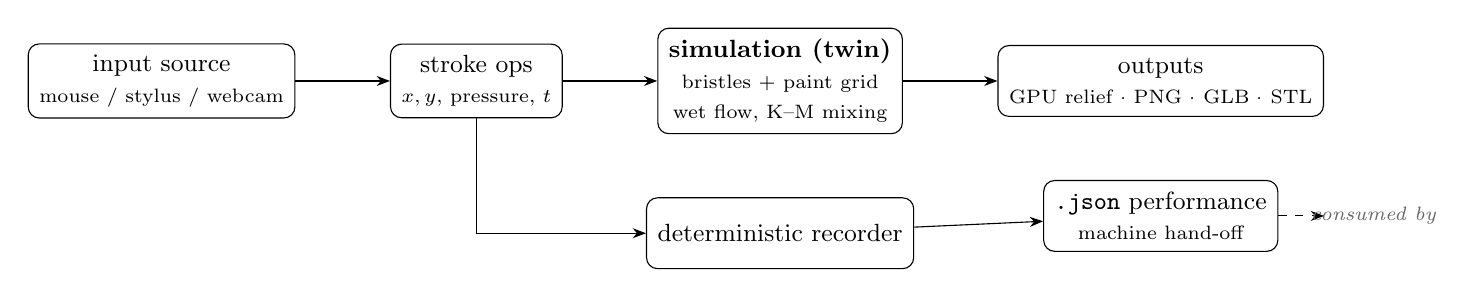
\begin{tikzpicture}[
  node distance=8mm and 12mm, >={Stealth[]},
  box/.style={draw, rounded corners, align=center, inner sep=4pt, font=\small,
              minimum height=9mm},
  lbl/.style={font=\scriptsize\itshape, text=black!60}]
  \node[box] (in) {input source\\\scriptsize mouse / stylus / webcam};
  \node[box, right=of in] (ops) {stroke ops\\\scriptsize $x,y$, pressure, $t$};
  \node[box, right=of ops] (sim) {\textbf{simulation (twin)}\\\scriptsize bristles $+$ paint grid\\\scriptsize wet flow, K--M mixing};
  \node[box, right=of sim] (out) {outputs\\\scriptsize GPU relief · PNG · GLB · STL};
  \node[box, below=of sim] (rec) {deterministic recorder};
  \node[box, below=of out] (perf) {\code{.json} performance\\\scriptsize machine hand-off};
  \draw[->] (in) -- (ops);
  \draw[->] (ops) -- (sim);
  \draw[->] (sim) -- (out);
  \draw[->] (ops) |- (rec);
  \draw[->] (rec) -- (perf);
  \draw[->, dashed] (perf) -- node[lbl, right]{consumed by} (out.south east|-perf.east) ;
\end{tikzpicture}
\caption{The pipeline. Input becomes a stroke-op stream that drives the paint
simulation (the twin) and, in parallel, a deterministic recorder that emits the
machine-agnostic \code{.json} performance. A separate machine driver (not in this
system) would consume that performance to paint physically.}
\label{fig:pipeline}
\end{figure}

\paragraph{Brush and paint.} The brush is a head of \num{80} spring-mass bristles
(defaults from the model reference), each a tip that lags a moving, splaying
anchor under semi-implicit Euler; contact is a pressure-flattened
\emph{segment} (belly-leading, tip-trailing) so marks emerge from motion rather
than stamping. Each bristle carries a finite load that drains to drybrush.
Deposition writes a soft dab into per-cell \code{Float32List} fields
(\code{thickness}, \code{r,g,b}, \code{wet}), gated by the canvas tooth for
scumble. Pigments combine subtractively via Kubelka--Munk in K/S space
\citep{haase1992pigment,sochorova2021pigment}. These choices follow
\citet{baxter2004impasto} and \citet{chen2015wetbrush} and are documented, with
constants, in the repository's model reference.

\paragraph{Conservative wet flow.} Each frame a flow step runs over the wet
bounding box only. Leveling (a downhill push to the 4-neighbourhood) and a body
force (gravity and/or spin) each draw paint from a cell; because their \emph{sum}
can exceed what the cell holds, the step first collects all requested outflow and,
if it exceeds a fraction of the cell's contents, scales the whole set by one
factor --- a per-cell \emph{joint outflow budget}. Nothing leaves a cell that was
not there, so the field is mass-conservative and cannot manufacture paint or
diverge (Section~\ref{sec:eval}). Colour and wetness advect mass-weighted with the
moving paint. Drips use a yield-stress (Bingham) rule: only thickness above a
yield film is mobile, so paint holds its shape until gravity overcomes the
threshold.

\paragraph{Rotating-frame body force (spin).}
\label{sec:spin}
Gravity is a uniform drift vector; spinning the canvas replaces it with a
\emph{position-dependent} one. In the co-rotating frame a cell at offset
$\mathbf{r}=(x-c_x,\,y-c_y)$ from the pivot feels a centrifugal drift
$\propto \omega^2\mathbf{r}$ (outward, zero at the pivot) plus a Coriolis term
$\propto \omega$ (perpendicular, signed by direction):
\[
  d g_x = g_x + s_{\mathrm{cf}}(x-c_x) + s_{\mathrm{cor}}(y-c_y), \qquad
  d g_y = g_y + s_{\mathrm{cf}}(y-c_y) - s_{\mathrm{cor}}(x-c_x),
\]
with $s_{\mathrm{cf}}\propto\omega^2$, $s_{\mathrm{cor}}\propto\omega$. This runs
through the \emph{same} yield-stress, joint-budget path as gravity, so spin stays
conservative at any rate. Our prior-art survey found no academic graphics system
that adds rotating-frame body forces to a conservative wet-paint field; we report
this as a minor secondary contribution (Figure~\ref{fig:spin}).

\begin{figure}[t]
\centering
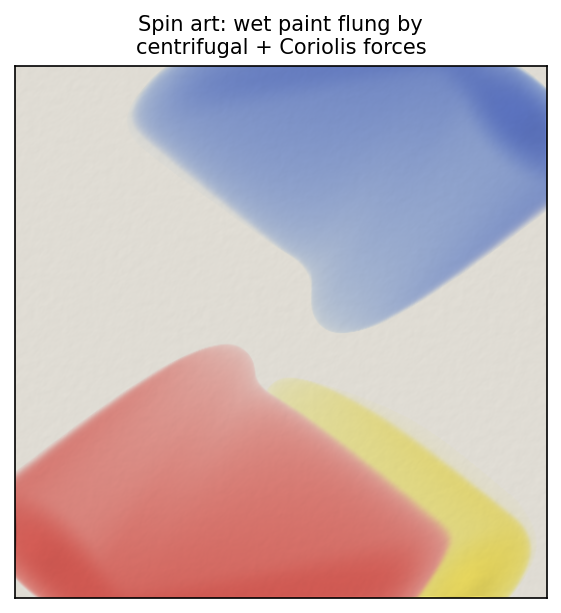
\includegraphics[width=0.48\linewidth]{figures/spinart.png}
\caption{Spin art from the rotating-frame body force: three wet paint blobs
flung outward and curled tangentially (Coriolis) by 420 conservative flow
substeps at a fixed rate. Simulated height$+$albedo, rendered offline.}
\label{fig:spin}
\end{figure}

\section{The performance interface}
\label{sec:interface}

The artifact that crosses the simulator/machine boundary is a
\code{TwinPerformance}: a versioned, ordered list of timestamped operations ---
\code{down}, \code{move}, \code{up}, and \code{reload} --- each carrying only
\emph{intent}. A \code{down}/\code{move} carries grid position $x,y$ and a
contact \code{pressure} in $[0,1]$; \code{reload} carries the loaded pigment as
linear RGB. Coordinates are grid cells with an optional millimetre hint
(\code{sizeMm}) for physical size; pressure is defined to map to a machine's
Z/force mechanism, which the machine owns. The design decision (recorded as an
architecture decision in the repository) is that the simulator emits this artifact
and contains \emph{no} kinematics, firmware, G-code dialect, Z-mechanism mapping,
paint-well coordinates, or calibration --- a downstream driver owns all of that.
The performance encodes intent so that authoring tool and machine can evolve
independently, and so the same artifact can target different machines.

\section{The twin: deterministic replay}
\label{sec:twin}

Because a machine must execute a fixed description, the performance must specify
the painting reproducibly. The operation stream is deterministic and round-trips
losslessly through JSON (verified headlessly); velocity-dependent deposition
(``dwell'') is reconstructed from recorded timestamps rather than wall-clock, so
the authored intent replays faithfully. \textbf{Honest caveat:} the wet-flow step
is advanced with real-time frame deltas, so an in-application \emph{replay} of a
performance reproduces the painting only \emph{approximately}, not bit-for-bit;
the authoritative object is the op stream, and exact reproduction would require
advancing flow on a fixed timestep keyed to op time. We treat that fixed-timestep
flow as required work to make the twin bit-exact (Section~\ref{sec:limits}).

\begin{figure}[t]
\centering
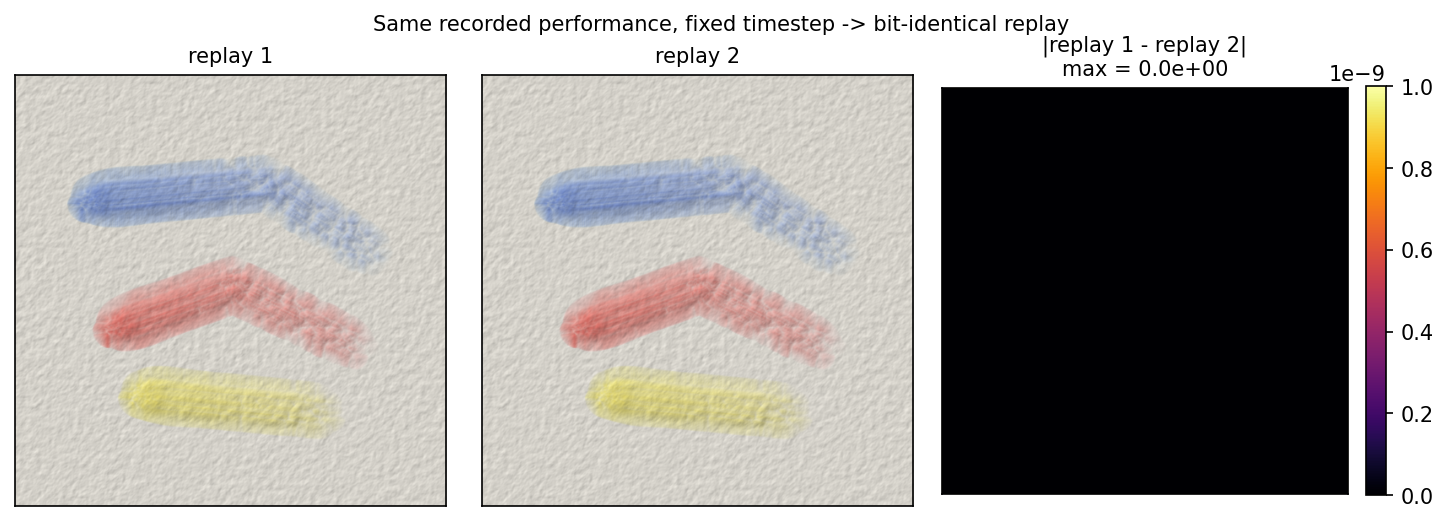
\includegraphics[width=\linewidth]{figures/determinism.png}
\caption{Op-stream determinism. The same recorded performance replayed twice
through the sim on a \emph{fixed} timestep yields bit-identical height fields
(right: $\max|\Delta|=0$). Under the real-time timestep used interactively the
reproduction is only approximate; a fixed timestep makes it exact.}
\label{fig:det}
\end{figure}

\section{Dual-use impasto height field}
\label{sec:dual}

A height-field paint model represents the painting as a relief surface. The same
\code{thickness}$+$\code{canvasHeight} field that the GPU shades on screen is
exported as geometry: a watertight binary STL (relief top, flat base, joining
side walls) and a vertex-coloured GLB, both at real-world millimetre scale (the
user sets the longer-side size, peak relief height, and base thickness). Preview
and fabrication geometry are therefore a single representation rather than two
pipelines that must be kept in agreement. The height-field-to-solid step itself is
commodity (cf. lithophanes) and is not the contribution; the point is that the
field is produced \emph{inside the authoring act} by the paint simulation, so no
scanning of a physical original (cf. \citealp{elkhuizen2019reproducing}) and no
bas-relief depth compression (cf. \citealp{weyrich2007basrelief,kerber2012survey})
are needed.

\begin{figure}[t]
\centering
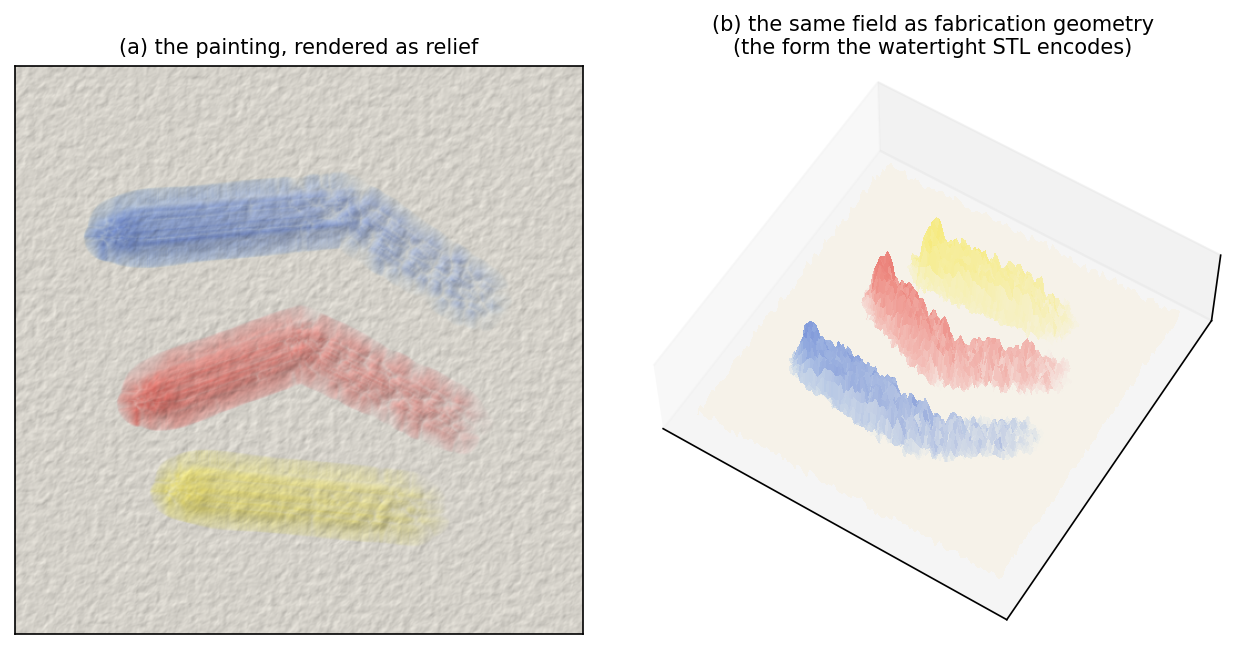
\includegraphics[width=\linewidth]{figures/dualgeometry.png}
\caption{The dual-use height field. (a) the painting rendered as relief;
(b) the \emph{same} simulated field as a 3D surface --- the form the watertight
STL export encodes --- coloured by the same pigment. One representation serves
both preview and fabrication. Rendered offline from the sim fields.}
\label{fig:dual}
\end{figure}

\section{Evaluation (simulation-validated)}
\label{sec:eval}

We state the evidence class of each check explicitly. All are
\emph{internal-consistency / simulation} results; none is an external, physical
validation.
\begin{itemize}
\item \textbf{Conservation and stability (simulated).} An aggressive
  diagonal-drip stress test runs \num{600} steps and remains finite with mass
  conserved to floating-point exactness --- the joint-budget invariant holds even
  for runny paint on a steep tilt.
\item \textbf{Spin behaviour (simulated).} An off-centre wet blob migrates to the
  rim; a centred blob flings into a ring while its centroid stays pinned at the
  pivot; mass is conserved. This is an internal consistency check that the
  rotating-frame force behaves as derived, not a claim about physical spin art.
\item \textbf{Determinism (simulated).} The performance stream round-trips
  through JSON and replays deterministically at the op level, subject to the
  wet-flow timing caveat of Section~\ref{sec:twin}.
\item \textbf{Watertight export (simulated).} The STL writer produces a closed
  two-manifold solid (checked by the export test), a prerequisite for slicing and
  fabrication.
\end{itemize}
Two independent implementations agreeing, or a simulator agreeing with itself on
replay, is internal consistency --- \emph{not} evidence that a machine would
reproduce the painting. That is the gap Section~\ref{sec:future} sets out to
close.

\section{Limitations}
\label{sec:limits}

\begin{itemize}
\item \textbf{No physical demonstrator (the central open item).} No machine has
  executed a performance. The claim that this interface yields a faithful
  physical painting is \emph{unvalidated}; there is no physical $n$.
\item \textbf{Replay is approximate, not bit-exact.} Wet flow uses real-time
  frame deltas; the op stream is deterministic but the reproduced painting is
  not. Fixed-timestep flow keyed to op time would close this.
\item \textbf{Uncalibrated constants (quarantined by name).} Every physical-looking
  number is a first-cut authored value, not calibrated to a real brush or paint:
  deposition rate ($2.2$), yield film (\code{dripYield}$=0.07$), viscosity
  coupling, the spin coefficients ($s_{\mathrm{cf}},s_{\mathrm{cor}}$), and the
  export mapping (the STL \code{paintWeight}$=3.0$ relief exaggeration and the
  \code{mmPerCell} scale). These would be calibrated by matching simulated to
  photographed strokes of a real brush/paint (the repository's modelling note
  sketches this, with the machine as the data-collection rig).
\item \textbf{Pressure$\rightarrow$Z is asserted.} The mapping from contact
  pressure to a physical Z/force mechanism is defined by the interface but not
  characterised against real hardware.
\item \textbf{Deposition gaps.} Pour (no-brush) deposition is captured as a
  toolpath but not yet reproduced on replay; deposition is per-distance rather
  than time-in-contact (a more principled model is future work).
\item \textbf{The ``twin'' is currently one-directional.} The virtual side
  authors the physical; nothing physical yet feeds back to calibrate the virtual.
  A twin in the strict, bidirectional sense
  \citep{grieves2017twin,glaessgen2012twin} awaits the feedback loop of
  Section~\ref{sec:future}; until then this is closer to direct digital
  manufacturing.
\item \textbf{The simulation is not novel.} Its value here is as a faithful,
  open, testable substrate behind the interface, not as a new paint model.
\end{itemize}

\section{Future directions}
\label{sec:future}

The concrete path, drawn from the project roadmap:
(1) \textbf{Close the loop} --- a minimal three-axis machine executes one recorded
performance, turning the central claim into a measured result (the arXiv \emph{v2}
upgrade, with a simulation-versus-physical fidelity comparison);
(2) \textbf{brush/paint calibration} against real strokes, retiring the
quarantined constants;
(3) \textbf{fixed-timestep flow} to make replay bit-exact;
(4) \textbf{live input} from depth-camera arm tracking through the same stroke
seam; and
(5) a \textbf{G-code emitter} that consumes the performance --- which, by the
interface design, lives in the separate machine project, not here.

\section{Conclusion}

The transferable discipline is to treat expressive fabrication as a
\emph{deterministic, replayable performance} authored by a physics simulator that
acts as the twin, with a clean boundary between recorded \emph{intent} and machine
\emph{kinematics}, and with the simulated relief doubling as fabrication geometry.
The paint physics here is not new; the factoring is. What remains --- and what
would convert this design paper into a fabrication result --- is to let a machine
execute a performance and to measure how close the physical painting comes to its
twin. The implementation is open source at
\url{https://github.com/dnuke-art/entropy-brush}.

\bibliographystyle{unsrtnat}
\bibliography{references}

\end{document}
